\documentclass[a5paper,10pt]{article}

%\usepackage{showframe}

\usepackage[spanish]{babel}
\usepackage[utf8]{inputenc}
\usepackage[T1]{fontenc}
\usepackage[]{times}
\usepackage[colorlinks=true]{hyperref}
\usepackage{graphicx}
%\usepackage{subcaption}
\usepackage{listingsutf8}
\usepackage{xcolor}

\addtolength{\voffset}{-2cm}
\addtolength{\textheight}{4cm}

\renewcommand{\lstlistingname}{Código}

% Código fuente tipo consola (shell)
\lstdefinestyle{consola}{
  backgroundcolor=\color{black},
  belowcaptionskip=1\baselineskip,
  frame=,
  xleftmargin=\parindent,
  language=bash,
  basicstyle=\footnotesize\ttfamily\color{white},
  commentstyle=\itshape\color{purple!40!black},
}


\author{Maximiliano A. Eschoyez}
\title{ANTLR en Visual Studio Code}
\date{2019}

\begin{document}
%\ebook
\maketitle

\begin{abstract}
	Esta guía tiene como fin explicar la utilización de ANTLR en la IDE Visual Studio Code.  Se explican los pasos mínimos desde la instalación de ANTLR y PJava hasta compilación de código fuente y la generación de diferentes gráficos de análisis.
\end{abstract}

\section{\emph{plug--in} ANTLR}
\label{intro}

En la \href{https://www.antlr.org/tools.html}{página web de ANTLR} se pueden encontrar los \emph{plug--in} para diferentes IDEs.

\begin{figure}[b]
	\centering
	
\includegraphics[width=3cm]{IconoANTLRvscode}
	\caption{ANTLR4 grammar syntax support -- Mike Lischke}
	\label{icono}
\end{figure}

Si bien para Visual Studio Code existen más herramientas para ANTLR, vamos a utilizar el \emph{plug--in} de Mike Lischke \href{https://marketplace.visualstudio.com/items?itemName=mike-lischke.vscode-antlr4}{ANTLR4 grammar syntax support}~(Figura~\ref{icono}).

El \emph{plug--in} completo se encuentra publicado con acceso libre en GitHub.  Este documento se basa en la documentación del \href{https://github.com/mike-lischke/vscode-antlr4/tree/master/doc}{\emph{plug--in ANTLR}}.



\section{Instalación del \emph{plug--in}}
\label{instalacion}

La instalación se puede realizar de dos formas:
\begin{enumerate}
	\item con el atajo de teclado \verb|Ctl+Shift+x| o \emph{clickeando} el ícono \emph{Extensions} y buscándolo, o
    \item con el atajo de teclado \verb|Ctl+p| para ejecutar en el \emph{VS Code Quick Open} el comando
    \begin{verbatim}
		ext install mike-lischke.vscode-antlr4
	\end{verbatim}
\end{enumerate}

\begin{center}
	\fbox{
		\parbox{.9\textwidth}{\textbf{NOTA}: Debe tenerse en cuenta que es necesario tener instalada la biblioteca ANTLR en el sistema o incluir el \texttt{.jar} en el proyecto. Sin alguna de esta alternativas, el \emph{plug--in} hará todo lo necesario pero no podremos generar código ejecutable.}
	}	
\end{center}


\section{¿Cómo vamos a trabajar?}

Vamos trabajar dentro de un proyecto Java de tipo Maven, por lo tanto, es necesario instalar soporte Java, particularmente el \emph{plug--in \textbf{Maven for Java}} (\verb|vscjava.vscode-maven|).  Para más información, ver la documentación \href{https://code.visualstudio.com/docs/java/java-project}{\emph{Java Project Management in VS Code}} de la página de Visual Studio Code.

\begin{figure}[p]
	\centering
	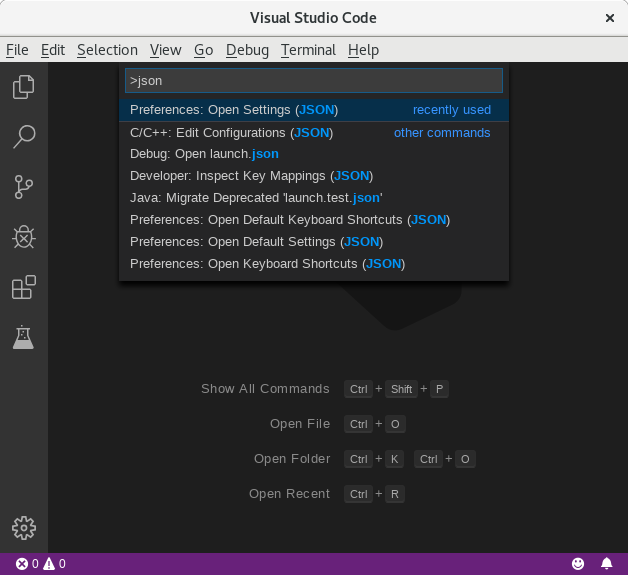
\includegraphics[width=.95\textwidth]{SelectJSON}
	\caption{Acceso a la configuración (archivo \texttt{settings.json}).}
	\label{preferences}
\end{figure}

Para simplificar la generación del software, vamos a colocar todos los archivos en el mismo paquete de Java.  Para esto, debemos modificar el archivo \verb|settings.json|.  Se puede acceder de varias formas, pero la más simple es siguiendo estos pasos:
\begin{enumerate}
	\item Abrir el \emph{Command Palette} con \verb|Ctl+Shift+P|,
	\item Buscar la opción \emph{Preferences: Open Settings (JSON)} y seleccionarla (Figura~\ref{preferences}),
	\item Agregar las siguientes líneas de código
	\begin{lstlisting}[style=consola]
	"antlr4.generation.mode": "external",
	"antlr4.generation.visitors": true
	\end{lstlisting}
\end{enumerate}
Hay que tener en cuenta que la coma es el separador en JSON y no debe faltar.  Además, las líneas de código deben estar antes de la llave de cierre como en el ejemplo del Código~\ref{settings}.

\lstinputlisting[float,style=consola,caption={Ejemplo de archivo \texttt{settings.json}.},label=settings]{settings.json}


\section{Primer Proyecto}
\label{primerproyecto}

Ya instalados y configurados los \emph{plug--ins} necesarios, podemos comenzar el primer proyecto.

\subsection{Crear Proyecto Java Maven}
\label{proyecto_maven}

\begin{figure}[t]
	\centering
	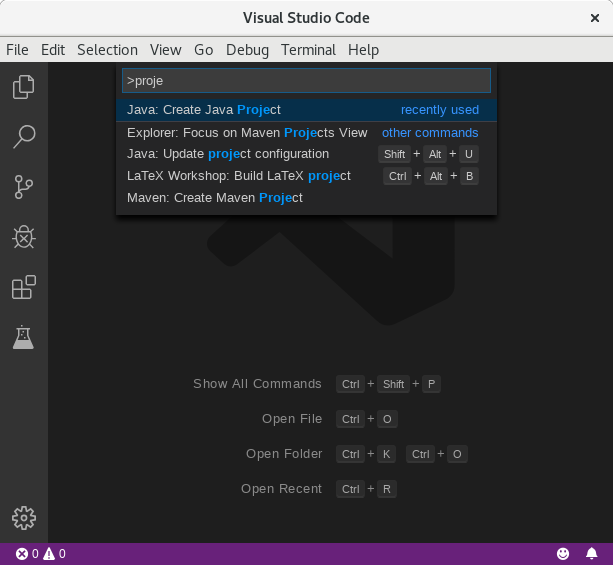
\includegraphics[width=.95\textwidth]{NuevoProyecto}
	\caption{Nuevo proyecto Java.}
	\label{maven_nuevo}
\end{figure}


El primer paso es crear un proyecto Java.  Para esto, se puede acceder al \emph{Command Palette} con el atajo \verb|Ctl+Shift+P|, escribir la palabra \emph{project} y elegir la opción ``\emph{Java: Create Java Project}'' (Fig.~\ref{maven_nuevo}). Luego, elegir la carpeta destino y darle nombre al proyecto.  Al finalizar estos pasos, tendremos un proyecto Java con un paquete por defecto denominado \verb|App|.  El archivo \verb|app.java| contiente el método \verb|main()| y está listo para compilar y ejecutar.


\begin{figure}[t]
	\centering
	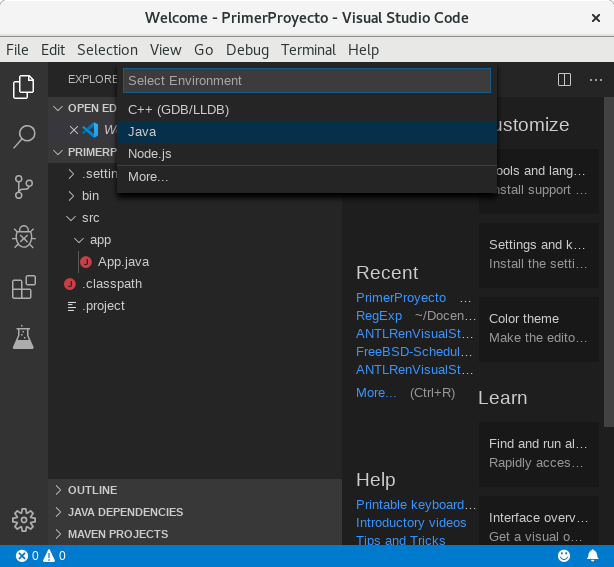
\includegraphics[width=.95\textwidth]{PrimerCompilacion}
	\caption{Elegir Java para compilar.}
	\label{java_project}
\end{figure}

\begin{figure}[t]
	\centering
	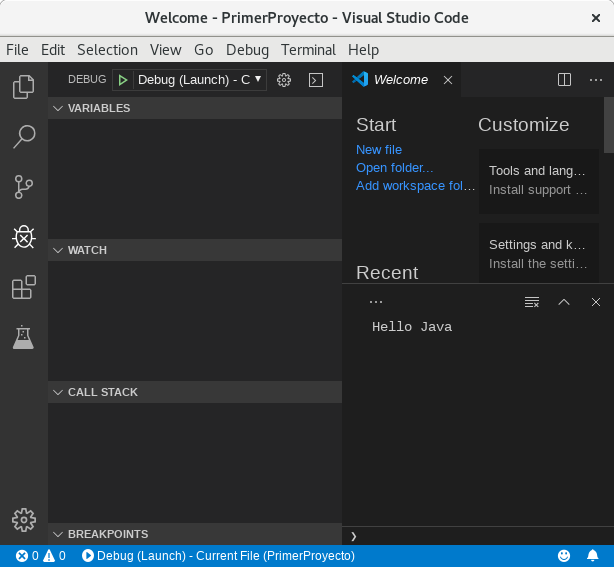
\includegraphics[width=.95\textwidth]{PrimeraEjecucion}
	\caption{Nombrar proyecto Java.}
	\label{hello_java}
\end{figure}


Recordemos que Visual Studio Code está pensado para desarrollar software, por lo tanto, cuando querramos ejecutar nuestro software vamos a hacerlo sobre el \emph{debugger}.  La ejecución se realiza presionando \verb|F5|.  La primera ejecución del proyecto necesita que se configuren parámetros de compilación qué, para nuestro caso, será suficiente con las configuraciones por defecto.  Al presionar \verb|F5| por primera vez debemos elegir ``Java'' como tipo de proyecto  (Fig.~\ref{java_project}).  Esta acción crea y abre el archivo de configuración \verb|launch.json| en la carpeta \verb|.vscode| del proyecto.  Si presionamos nuevamente \verb|F5| se ejecutará el proyecto y veremos que se abre el panel del \emph{debugger} y se muestra la salida por consola con el texto ``\emph{Hello Java}'' (Fig.~\ref{hello_java}).  Las próximas veces se ejecutará nuestro programa sin necesidad de realizar configuraciones adicionales.


\subsection{Archivo ANTLR}
\label{archivo_antlr}

Con el proyecto Java creado y listo para trabajar vamos a crear el archivo para ANTLR. Los archivos de ANTLR llevan extensión \verb|.g| o \verb|.g4|, pero utilizaremos la segunda opción.  El atajo de teclado para crear un archivo vacío es \verb|Ctl+n|, que para hacer efectivo el coloreo hay que guardarlo (\verb|Ctl+s|) con la extensión apropiada.

ANTLR permite la generación del \emph{lexer} y del \emph{parser}.  Por lo tanto, los archivos \verb|.g4| pueden ser para el primero, el segundo o ambos combinados.  Nosotros utilizaremos archivos combinados dentro del paquete que contiene el método \verb|main()| para facilitar la ejecución y visualización de resultados.  En particular, en el proyecto ejemplo guardaremos el archivo \verb|.g4| en la carpeta \verb|src/app/|.


\end{document}
